\documentclass[12pt,a4paper]{article}

\usepackage[T2A]{fontenc}
\usepackage[utf8]{inputenc}
\usepackage[bulgarian,english]{babel}
\usepackage{geometry}
\usepackage{graphicx}
\usepackage{float}
\usepackage{placeins}
\usepackage{booktabs}
\usepackage{array}
\usepackage{amsmath}
\usepackage{amssymb}
\usepackage{setspace}
\usepackage{caption}
\usepackage{subcaption}
\usepackage{csquotes}
\usepackage{multicol}
\usepackage{tikz}
\usetikzlibrary{arrows.meta, positioning, fit, calc, shapes.geometric, shapes.misc, shapes.symbols, backgrounds}
\usepackage{pgfplots}
\usepackage{fontawesome5}
\pgfplotsset{compat=1.18}
\usepackage{hyperref}
\usepackage{cleveref}

\geometry{margin=2.5cm}
\setstretch{1.2}
\captionsetup[table]{position=bottom}
\captionsetup{font=small}
% let floats share pages with text instead of leaving half-empty pages
\renewcommand{\topfraction}{0.85}
\renewcommand{\bottomfraction}{0.6}
\renewcommand{\textfraction}{0.1}
\renewcommand{\floatpagefraction}{0.8}
\setcounter{totalnumber}{4}
\hypersetup{
    colorlinks=true,
    linkcolor=black,
    citecolor=black,
    urlcolor=blue
}

% Bulgarian quotation marks and cross-reference names
\DeclareQuoteStyle{bulgarian}{\quotedblbase}{\textquotedblleft}{\quotesinglbase}{\textquoteleft}
\setquotestyle{bulgarian}
\crefname{figure}{фиг.}{фиг.}
\Crefname{figure}{Фиг.}{Фиг.}
\crefname{table}{табл.}{табл.}
\Crefname{table}{Табл.}{Табл.}
\crefname{section}{раздел}{раздели}
\Crefname{section}{Раздел}{Раздели}
\crefname{subsection}{раздел}{раздели}
\Crefname{subsection}{Раздел}{Раздели}
\crefname{equation}{формула}{формули}
\Crefname{equation}{Формула}{Формули}

\title{Курсов проект по дисциплината Информационни технологии в медицината}
\author{Асен Пантелеев Попов}
\date{2026}

\begin{document}

\begin{titlepage}
\thispagestyle{plain}

\noindent
\begin{minipage}{0.17\textwidth}
    
\includegraphics[width=\linewidth]{3_TU_bg_n.png}
\end{minipage}%
\hspace{0.03\textwidth}%
\begin{minipage}{0.8\textwidth}
    \raggedright
    \large
    \textbf{ТЕХНИЧЕСКИ УНИВЕРСИТЕТ – СОФИЯ}\\[-0.3ex]
    \rule{\linewidth}{0.2pt}\\[-0.6ex]
    \textbf{ФАКУЛТЕТ КОМПЮТЪРНИ СИСТЕМИ И ТЕХНОЛОГИИ}\\[0.2cm]
\end{minipage}

\vspace{3cm}

\begin{center}
    \textbf{\LARGE КУРСОВ ПРОЕКТ}\\[1cm]

    \normalsize
    Дисциплина: Информационни технологии в медицината\\[0.8cm]

    \textbf{Тема:}\\[0.3cm]
    \textbf{Проектиране на електрокардиографски апарат\\
    с компресия на ЕКГ сигнала чрез\\
    едномерен конволюционен автоенкодер}\\[2.8cm]
\end{center}

\vspace{0.8cm}

\begin{flushleft}
\textbf{Изготвил:}\\
Асен Пантелеев Попов\\
Фак. № 121223246\\
Група 38\\
IV курс, КСИ\\
e-mail: \texttt{asepopov@tu-sofia.bg}
\end{flushleft}

\vspace{1.2cm}

\begin{flushleft}
\textbf{Ръководител:}\\
доц. д-р инж. Калин Димитров
\end{flushleft}

\vfill

\begin{center}
София, 2026 г.
\end{center}

\end{titlepage}

\selectlanguage{bulgarian}

\begin{spacing}{1.0}
\tableofcontents
\end{spacing}
\newpage

% =====================================================================
\section{Увод}
Електрокардиограмата (ЕКГ) е един от най-широко използваните неинвазивни методи за диагностика в медицината. Тя регистрира електрическата активност на сърцето чрез електроди, поставени върху кожата, и позволява да се оценят сърдечният ритъм, проводимостта и редица патологични състояния. С развитието на преносимите и носимите устройства все по-често ЕКГ се записва продължително, извън болничната среда, и се предава безжично към компютър, смартфон или облачна услуга. Това поставя два практически въпроса: как да се проектира компактен и безопасен апарат за регистриране на сигнала и как да се намали обемът на данните, които трябва да бъдат предадени или съхранени, без да се загуби съществена информация за формата на сигнала.

Основната част на проекта е разработването на алгоритъм за компресия на ЕКГ сигнала чрез едномерен конволюционен автоенкодер (1D Convolutional Autoencoder, CAE), който преобразува всеки прозорец от 256 отчета в кратък латентен вектор от 8, 16 или 32 числа и след това възстановява сигнала от него. Алгоритъмът е обучен и оценен върху публичния набор от данни PTB-XL \cite{wagner2020ptbxl,wagner2022ptbxlphysionet}, а качеството на реконструкцията е измерено чрез стандартните показатели PRD и PRDN. Допълнително е представена концепция за вграждането на алгоритъма в едноканален електрокардиографски апарат, изграден около аналоговия преден блок ADS1292R на Texas Instruments и микроконтролера ESP32-S3 на Espressif.

Изследователският въпрос на проекта е как размерът на латентния вектор влияе върху качеството на реконструкцията и степента на компресия и дали обученият енкодер може да бъде изпълнен в реално време от ресурсно ограничен микроконтролер. Основният резултат е крайна конфигурация с латентен вектор от 32 числа, която постига медиана на PRDN 18.7\% върху тестовия дял при каузална филтрация и int8 представяне на латентния вектор, при идеализирана степен на компресия 16:1. Енкодерът съдържа около 79 хиляди параметъра и по оценка изисква по-малко от 1\% от наличното изчислително време на ESP32-S3.

Проектът е изследователски и инженерен демонстратор, а не сертифицирано медицинско изделие. Реалното свързване на експериментална схема към човек изисква спазване на изискванията за електрическа безопасност (IEC 60601-1 \cite{iec60601}), галванична изолация и верификация, които са извън обхвата на работата.

% =====================================================================
\section{Теоретична основа}

\subsection{Електрическа активност на сърцето и ЕКГ сигналът}
Съкращението на сърдечния мускул се предизвиква от електрически импулс, който възниква в синусовия възел, разпространява се през предсърдията, преминава през атриовентрикуларния възел и достига камерите чрез снопа на Хис и Пуркиниевите влакна. Деполяризацията и реполяризацията на мускулните клетки създават променливо електрическо поле, чийто проекции върху повърхността на тялото се регистрират като ЕКГ \cite{webster2010medical}. Един сърдечен цикъл съдържа няколко характерни вълни (\cref{fig:ecg_beat}): P вълната отразява деполяризацията на предсърдията, QRS комплексът -- бързата деполяризация на камерите, а T вълната -- тяхната реполяризация. Интервалите между вълните (PR, QRS, QT) и нивото на ST сегмента имат пряко диагностично значение.

\begin{figure}[htbp]
    \centering
    % Stylised single ECG cycle (sum of Gaussians) with the characteristic waves and intervals.
\begin{tikzpicture}
  \begin{axis}[
      width=0.85\textwidth, height=4.6cm,
      xmin=0, xmax=0.9, ymin=-0.62, ymax=1.25,
      axis lines=left, axis line style={gray},
      xlabel={време (s)}, ylabel={mV},
      xtick={0,0.2,0.4,0.6,0.8}, ytick={0,0.5,1},
      tick label style={font=\footnotesize, /pgf/number format/assume math mode=true},
      label style={font=\footnotesize},
      clip=false,
    ]
    \addplot[black, thick, samples=600, domain=0:0.9]
      {0.15*exp(-((x-0.18)/0.03)^2) - 0.12*exp(-((x-0.355)/0.009)^2)
       + 1.05*exp(-((x-0.38)/0.011)^2) - 0.30*exp(-((x-0.405)/0.010)^2)
       + 0.32*exp(-((x-0.62)/0.05)^2)};
    % wave labels
    \node[font=\small] at (axis cs:0.18,0.27) {P};
    \node[font=\small] at (axis cs:0.335,-0.17) {Q};
    \node[font=\small] at (axis cs:0.38,1.16) {R};
    \node[font=\small] at (axis cs:0.428,-0.36) {S};
    \node[font=\small] at (axis cs:0.62,0.43) {T};
    % intervals
    \draw[<->, gray] (axis cs:0.13,0.62) -- node[above, font=\scriptsize, text=black] {PR интервал} (axis cs:0.345,0.62);
    \draw[<->, gray] (axis cs:0.345,-0.53) -- (axis cs:0.425,-0.53);
    \node[font=\scriptsize, anchor=west] at (axis cs:0.43,-0.53) {QRS комплекс (\(\approx\)0.08--0.10 s)};
    \draw[<->, gray] (axis cs:0.345,0.85) -- node[above, font=\scriptsize, text=black] {QT интервал} (axis cs:0.68,0.85);
    \draw[<->, gray] (axis cs:0.425,0.12) -- node[above, font=\scriptsize, text=black] {ST сегмент} (axis cs:0.565,0.12);
  \end{axis}
\end{tikzpicture}

    \caption{Схематично представяне на един сърдечен цикъл с характерните вълни P, Q, R, S, T и основните интервали.}
    \label{fig:ecg_beat}
\end{figure}

Повърхностният ЕКГ сигнал има амплитуда от порядъка на 0.5--4 mV, а честотното му съдържание за диагностични цели е в диапазона приблизително от 0.05 до 150 Hz \cite{kligfield2007aha}. Сигналът се наслагва върху значително по-големи смущения: постоянно напрежение на поляризация на електродите, което може да достигне стотици миливолта, бавен дрейф на изолинията, предизвикан от дишането и движението, мускулни артефакти и индуцирано мрежово напрежение с честота 50 Hz. Именно тези смущения определят изискванията към апаратната част и към цифровата обработка.

\subsection{Отвеждания и избор на отвеждане II}
Отвеждането описва двойката точки, между които се измерва потенциалната разлика. При класическите крайникови отвеждания на Айнтховен електродите се поставят на дясната ръка (RA), лявата ръка (LA) и левия крак (LL), а дясният крак (RL) се използва като референтен електрод (\cref{fig:einthoven}). Стандартната 12-канална ЕКГ добавя усилени крайникови и гръдни отвеждания и изисква по-сложен преден блок.

\begin{figure}[htbp]
    \centering
    % Einthoven triangle with the limb leads; lead II highlighted, plus the ADS1292R channel mapping.
\begin{tikzpicture}[
    el/.style={circle, draw, thick, minimum size=9mm, font=\small, fill=white},
    lead/.style={-{Stealth[length=2.5mm]}, thick, gray},
    lead2/.style={-{Stealth[length=3mm]}, very thick, blue!70!black},
  ]
  \node[el] (RA) at (0,3.2) {RA};
  \node[el] (LA) at (4.4,3.2) {LA};
  \node[el] (LL) at (2.2,0) {LL};
  \node[el, dashed] (RL) at (-0.6,0) {RL};

  \draw[lead] (RA) -- node[above, font=\small, text=black] {I} (LA);
  \draw[lead2] (RA) -- node[left, font=\small, text=blue!70!black] {II} (LL);
  \draw[lead] (LA) -- node[right, font=\small, text=black] {III} (LL);

  \node[font=\footnotesize, align=left, anchor=west] at (5.4,2.6)
    {\(\mathrm{I} = \Phi_{LA} - \Phi_{RA}\)\\[2pt]
     \(\mathbf{II} = \Phi_{LL} - \Phi_{RA}\)\\[2pt]
     \(\mathrm{III} = \Phi_{LL} - \Phi_{LA}\)};
  \node[font=\footnotesize, align=left, anchor=west] at (5.4,0.7)
    {ADS1292R, канал 2:\\
     LL \(\rightarrow\) IN2P,\; RA \(\rightarrow\) IN2N\\
     RL \(\leftarrow\) RLDOUT (активна референция)};
\end{tikzpicture}

    \caption{Триъгълник на Айнтховен и крайниковите отвеждания. Отвеждане II, използвано в проекта, измерва разликата между левия крак и дясната ръка и се подава на канал 2 на ADS1292R.}
    \label{fig:einthoven}
\end{figure}

В проекта е използвано само отвеждане II. То обикновено има най-ясно изразени P вълни и висок QRS комплекс, поради което е стандартният избор за мониторинг на ритъма. Изборът е съобразен и с апаратната част: двуканалният ADS1292R не може да регистрира 12 независими отвеждания, а за пълна 12-канална ЕКГ би бил необходим например осемканалният ADS1298 с подходяща конфигурация на електродите.

\subsection{Аналогов преден блок на електрокардиограф}
Аналоговият преден блок усилва сигнал от порядъка на миливолти, наслоен върху голямо синфазно смущение и постоянно отместване на електродите. Затова ключовите му характеристики са висок коефициент на потискане на синфазния сигнал (Common-Mode Rejection Ratio, CMRR), висок входен импеданс и нисък собствен шум \cite{webster2010medical}. Синфазното смущение допълнително се намалява чрез задвижване на десния крак (Right Leg Drive, RLD): усилвател подава към тялото през електрода RL инвертираното средно синфазно напрежение на входовете. Съвременните интегрални решения, като избрания в проекта ADS1292R, обединяват в един корпус програмируем усилвател, делта-сигма аналогово-цифров преобразувател (АЦП) с висока разделителна способност, RLD усилвател и детекция на откачен електрод, така че цялата филтрация може да се извърши цифрово.

\subsection{Компресия на ЕКГ сигнала и автоенкодери}
Компресията на ЕКГ намалява обема на данните при продължителен запис, безжично предаване или съхранение. Класическите методи се делят на директни методи във времевата област, методи с преобразувания (дискретно косинусово и уейвлет преобразуване) и параметрични методи. Компресията със загуби се оценява чрез степента на компресия и чрез изкривяването на реконструирания сигнал.

Автоенкодерът е невронна мрежа, която се обучава да възпроизвежда входа си през тясно място -- латентен вектор с малка размерност \cite{hinton2006reducing}. Енкодерът изобразява входния прозорец \(x\) в латентен вектор \(z = f_\theta(x)\), а декодерът възстановява \(\hat{x} = g_\phi(z)\). Параметрите се обучават чрез минимизиране на средноквадратичната грешка между \(x\) и \(\hat{x}\). За разлика от анализа на главните компоненти (PCA), който намира най-доброто линейно подпространство, автоенкодерът с нелинейни активации може да научи нелинейно многообразие. Това е съществено за ЕКГ, тъй като положението на сърдечните удари в прозореца се променя, а линейната база трудно описва такова отместване. Едномерните конволюции са естествен избор за времеви сигнали: те използват едни и същи тегла по цялата дължина на прозореца и затова са компактни и подходящи за микроконтролери.

\subsection{Показатели за качество на реконструкцията}
Най-разпространеният показател за изкривяване при компресия на ЕКГ е процентната средноквадратична разлика (Percentage Root-mean-square Difference, PRD). Нека \(x\) е референтният прозорец, \(\hat{x}\) е реконструкцията му, а \(\bar{x}\) е средната стойност на \(x\):
\begin{equation}
    \mathrm{PRD} = 100 \cdot \frac{\lVert x - \hat{x} \rVert_2}{\lVert x \rVert_2}\ (\%),
    \qquad
    \mathrm{PRDN} = 100 \cdot \frac{\lVert x - \hat{x} \rVert_2}{\lVert x - \bar{x} \rVert_2}\ (\%).
    \label{eq:prd}
\end{equation}
PRD зависи от постоянната съставка на сигнала: ако записът съдържа отместване (например от АЦП), знаменателят нараства и PRD изглежда изкуствено нисък. Нормираният вариант PRDN премахва тази зависимост и затова е основният показател в проекта. И двата показателя са отношения, така че глобален мащабиращ коефициент се съкращава. По-ниската стойност е по-добра. Често цитирана класификация за PRD определя стойности под 2\% като \enquote{много добро} качество и 2--9\% като \enquote{добро} качество \cite{zigel2000wdd}. Тези граници са ориентировъчни и не заменят визуалната оценка на P, QRS и T морфологията.

Степента на компресия (Compression Ratio, CR) в проекта се изчислява идеализирано, като отношение между обема на един суров прозорец и обема на латентния вектор:
\begin{equation}
    \mathrm{CR} = \frac{N \cdot b_x}{d \cdot b_z},
    \label{eq:cr}
\end{equation}
където \(N = 256\) е дължината на прозореца, \(b_x = 16\) бита е разрядността на суровия отчет, \(d\) е размерността на латентния вектор, а \(b_z = 8\) бита е разрядността на квантувания латентен елемент. При \(d = 32\) се получава \(\mathrm{CR} = 4096/256 = 16\). Оценката не включва заглавни части на пакетите и паметта за модела, които са общи за цялата сесия.

% =====================================================================
\section{Набор от данни}
\label{sec:data}
PTB-XL v1.0.3 съдържа 21\,799 клинични 12-канални ЕКГ записа с продължителност 10 s от 18\,869 пациенти \cite{wagner2020ptbxl,wagner2022ptbxlphysionet}. Записите са налични с честота 500 Hz и в понижена версия със 100 Hz, във формат WFDB с разделителна способност 1 \(\mu\)V. Наборът е публикуван в PhysioNet \cite{goldberger2000physionet} и е широко използван за оценка на алгоритми за анализ на ЕКГ \cite{strodthoff2021deep}. Метаданните съдържат диагностични твърдения на ниво запис и анотации за качеството на сигнала (дрейф на изолинията, статичен шум, импулсни смущения, проблеми с електродите). Тези анотации са използвани в проекта за анализ на грешките, а диагнозите не са необходими, тъй като автоенкодерът се обучава без етикети.

Разделянето на данните следва препоръката на авторите на набора: дялове 1--8 за обучение, дял 9 за валидация и дял 10 за тестване (\cref{tab:split}). Разделянето е на ниво пациент и се извършва преди разделянето на прозорци, така че прозорци от един и същ запис никога не попадат в различни дялове. Програмата проверява автоматично, че няма пациент в повече от един дял.

В проекта се използват 100-херцовите записи и само отвеждане II. Тази честота изисква уточнение по отношение на апаратната част, тъй като ADS1292R не поддържа такава честота на дискретизация: най-ниската му честота е 125 SPS. Затова апаратът дискретизира с 500 SPS, а микроконтролерът намалява честотата 5 пъти след цифров нискочестотен филтър. Това съответства на начина, по който са получени 100-херцовите записи в PTB-XL от оригиналните 500-херцови, и позволява моделът да бъде обучен директно върху данните от набора.

\begin{table}[htbp]
    \centering
    \begin{tabular}{l c c c c}
        \toprule
        Дял & \texttt{strat\_fold} & Записи & Пациенти & Прозорци \\
        \midrule
        Обучение & 1--8 & 17\,418 & 15\,023 & 104\,508 (стъпка 128) \\
        Валидация & 9 & 2\,183 & 1\,942 & 6\,549 (стъпка 256) \\
        Тест & 10 & 2\,198 & 1\,904 & 6\,594 (стъпка 256) \\
        \bottomrule
    \end{tabular}
    \caption{Разделяне на PTB-XL по пациенти и брой прозорци от 256 отчета във всеки дял.}
    \label{tab:split}
\end{table}

% =====================================================================
\section{Предварителна обработка на сигнала}

\subsection{Премахване на дрейфа на изолинията}
Дрейфът на изолинията е бавно изменение на нивото на сигнала, предизвикано основно от дишането и движението на електродите. Той се премахва с високочестотен IIR филтър на Бътъруърт от втори ред, реализиран като каскада от звена от втори ред (second-order sections, SOS) за числена устойчивост. Изследвани са две гранични честоти: 0.5 Hz, която премахва дрейфа ефективно, но може да изкриви ST сегмента, и 0.05 Hz, която съответства на препоръката на AHA за запазване на ST морфологията \cite{kligfield2007aha}, но премахва дрейфа значително по-слабо. За основните експерименти е избрана граничната честота 0.5 Hz.


Филтърът се прилага върху целия 10-секунден запис преди разделянето на прозорци. При ниски гранични честоти преходният процес на филтъра продължава няколко секунди и филтрацията на отделни 2.56-секундни прозорци би довела до силни изкривявания в началото на всеки прозорец.

\subsection{Филтрация с нулева фаза и каузална филтрация}
Офлайн обработката позволява филтрация с нулева фаза (\texttt{scipy.signal.sosfiltfilt} \cite{virtanen2020scipy}): сигналът се филтрира веднъж напред и веднъж назад във времето, при което фазовите закъснения на двете преминавания се компенсират и формата на вълните не се измества. Този подход използва бъдещи отчети и затова е невъзможен в устройство, което обработва сигнала в реално време. Апаратът може да използва само каузален филтър (\texttt{sosfilt}), при който изходът зависи само от текущия и предишните отчети. За да се избегне преходен процес от постоянното отместване в началото на записа, началното състояние на каузалния филтър се задава като установено състояние за първия отчет (\texttt{sosfilt\_zi}). Същата процедура трябва да бъде изпълнена и от фърмуера при стартиране.

\begin{figure}[htbp]
    \centering
    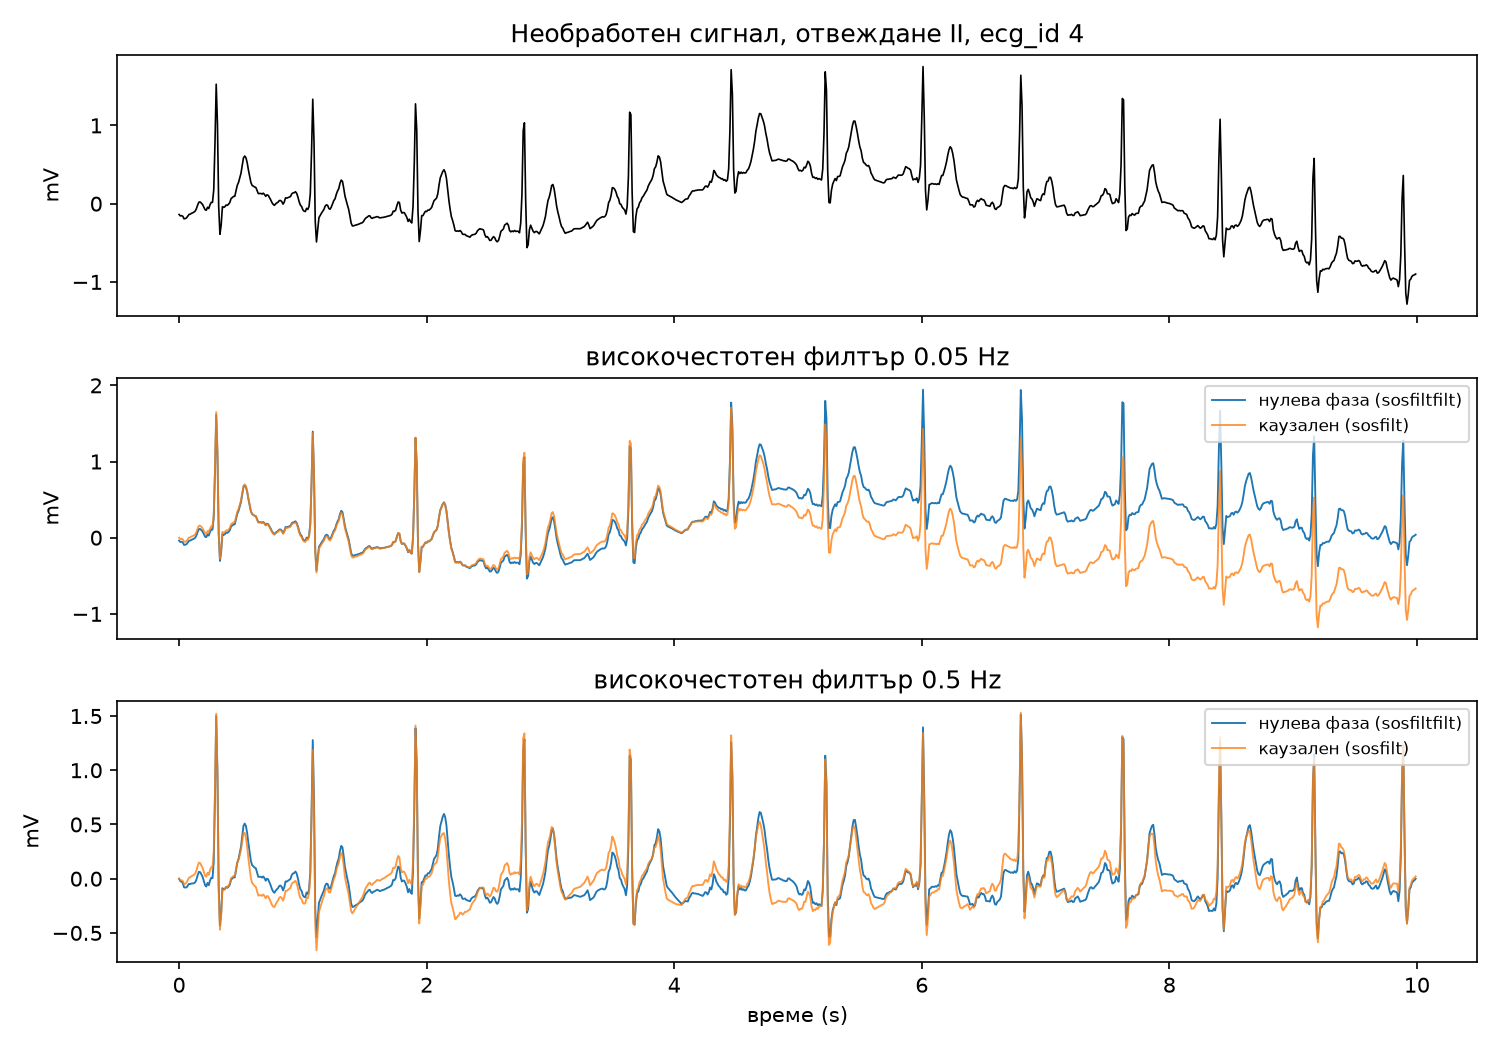
\includegraphics[width=0.92\textwidth]{../figures/filter_example.png}
    \caption{Запис от PTB-XL с изразен дрейф на изолинията (горе) и резултатът от филтрация с нулева фаза и каузална филтрация при 0.05 Hz и 0.5 Hz.}
    \label{fig:filter_example}
\end{figure}

\Cref{fig:filter_example} показва разликата между двата режима. При 0.05 Hz и двата филтъра оставят значителна част от дрейфа, като каузалният филтър го следва по-лошо. При 0.5 Hz дрейфът е премахнат, но каузалният филтър въвежда характерни понижения след QRS комплекса и T вълната и измества нивото на ST и TP сегментите. Това е типичното фазово изкривяване на каузалните високочестотни филтри, за което предупреждават стандартите за ЕКГ, и неговото влияние е измерено количествено в \cref{sec:causal}.

\subsection{Мащабиране и разделяне на прозорци}
След филтрацията сигналът се мащабира с един глобален коефициент \(s = 0.151\) mV, равен на стандартното отклонение на филтрирания сигнал в обучаващия дял. Използването на фиксиран коефициент вместо нормализация на всеки прозорец поотделно е съзнателно решение: при нормализация на прозорец към латентния вектор трябва да се предават и параметрите на нормализацията, което намалява степента на компресия. Фиксираният коефициент е константа, известна както на устройството, така и на приемника.

Филтрираните записи се разделят на прозорци от \(N = 256\) отчета (2.56 s). При обучение се използва стъпка 128 отчета (50\% застъпване), което дава 6 прозореца на запис и служи като увеличаване на данните. При оценка се използва стъпка 256, т.е. прозорци без застъпване, както би ги предавало устройството. Така застъпващите се и силно корелирани прозорци не увеличават изкуствено броя на тестовите примери, а показателите се отчитат и на ниво запис като медиана по прозорците на всеки запис.

% =====================================================================
\section{Модел и обучение}

\subsection{Архитектура на автоенкодера}
Финалната архитектура е показана на \cref{fig:cae}. Енкодерът се състои от три конволюционни слоя с ядро 5, стъпка 2 и допълване 2, всеки от които намалява дължината наполовина (\(256 \rightarrow 128 \rightarrow 64 \rightarrow 32\)), последвани от ReLU активация. Броят на каналите е \(16 \rightarrow 32 \rightarrow 64\) (ширина 16). Изходът с размер \(64 \times 32\) се преобразува във вектор и чрез линеен слой се проектира в латентния вектор \(z\). Латентният вектор и изходът на декодера нямат активационна функция, тъй като ЕКГ сигналът приема положителни и отрицателни стойности.

\begin{figure}[htbp]
    \centering
    \resizebox{\textwidth}{!}{% Architecture of the final 1D CAE (width 16, z = 32), in the style of the CG course paper:
% tensors drawn as blocks (height ~ length, width ~ channels), trapezia for Linear layers,
% latent vector as a stack of cells, dashed groups for where each half runs.
\begin{tikzpicture}[
  font=\footnotesize,
  >={Stealth[length=1.8mm]},
  arr/.style={->, thick, black!70},
  lbl/.style={font=\scriptsize, text=black!75, align=center},
  dim/.style={font=\scriptsize, text=black!70, align=center},
  thumb/.style={inner sep=0pt}]

  \colorlet{encC}{blue!55!cyan}
  \colorlet{decC}{orange!85!red}
  \colorlet{latC}{green!50!black}

  % tensor block: x-centre, height, width, colour, name, dimension label
  \newcommand{\tensor}[6]{%
    \fill[#4!12, draw=#4!45, line width=0.4pt, rounded corners=1pt]
      ($(#1,0)+(-#3/2+0.14,-#2/2+0.14)$) rectangle ($(#1,0)+(#3/2+0.14,#2/2+0.14)$);
    \fill[#4!20, draw=#4!60, line width=0.4pt, rounded corners=1pt]
      ($(#1,0)+(-#3/2+0.07,-#2/2+0.07)$) rectangle ($(#1,0)+(#3/2+0.07,#2/2+0.07)$);
    \node[draw=#4!80!black, fill=#4!30, line width=0.5pt, rounded corners=1pt,
          minimum height=#2 cm, minimum width=#3 cm, inner sep=0pt] (#5) at (#1,0) {};
    \node[dim] at (#1,-1.55) {#6};}

  % trapezium for a Linear layer: x-centre, left half-height, right half-height, colour, name
  \newcommand{\linear}[5]{%
    \fill[#4!15, draw=#4, line width=0.6pt, rounded corners=1.5pt]
      ($(#1,0)+(-0.45,#2)$) -- ($(#1,0)+(0.45,#3)$) -- ($(#1,0)+(0.45,-#3)$) -- ($(#1,0)+(-0.45,-#2)$) -- cycle;
    \coordinate (#5w) at ($(#1,0)+(-0.45,0)$);
    \coordinate (#5e) at ($(#1,0)+(0.45,0)$);
    \node[lbl, text=#4!60!black, font=\tiny] at (#1,0) {Linear};}

  % ---------------- input ----------------
  \node[thumb] (in) at (0,0) {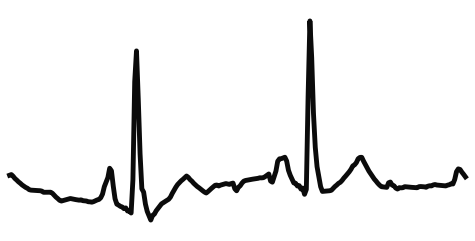
\includegraphics[width=2.3cm]{../figures/cae_in.png}};
  \node[lbl, below=1mm of in] {вход \(x\)\\\(1 \times 256\) (2.56 s)};

  % ---------------- encoder ----------------
  \tensor{2.1}{2.0}{0.30}{encC}{e1}{\(16 \times 128\)}
  \tensor{3.3}{1.45}{0.50}{encC}{e2}{\(32 \times 64\)}
  \tensor{4.55}{1.0}{0.75}{encC}{e3}{\(64 \times 32\)}
  \linear{5.9}{0.75}{0.42}{encC}{le}
  \draw[arr] (in) -- (e1);
  \draw[arr] (e1) -- (e2);
  \draw[arr] (e2) -- (e3);
  \draw[arr] (e3) -- (lew);

  % ---------------- latent vector ----------------
  \begin{scope}[shift={(7.15,0)}]
    \foreach \i in {0,...,7}
      \fill[latC!18!white, draw=latC!70!black, line width=0.3pt] (-0.15,-0.72+0.18*\i) rectangle (0.15,-0.56+0.18*\i);
  \end{scope}
  \coordinate (zw) at (7.0,0); \coordinate (ze) at (7.3,0);
  \node[lbl, text=latC!60!black] at (7.15,1.0) {\(z \in \mathbb{R}^{32}\)};
  \node[dim] at (7.15,-1.55) {32};
  \draw[arr] (lee) -- (zw);

  % ---------------- link: int8 latent ----------------
  \draw[arr, latC, line width=1pt] (ze) -- node[lbl, above, text=latC!60!black] {int8, 32 B} node[lbl, below, text=latC!60!black] {BLE / Wi-Fi} (9.95,0);

  % ---------------- decoder ----------------
  \linear{10.4}{0.42}{0.75}{decC}{ld}
  \tensor{11.75}{1.0}{0.75}{decC}{d1}{\(64 \times 32\)}
  \tensor{13.05}{1.45}{0.50}{decC}{d2}{\(32 \times 64\)}
  \tensor{14.3}{2.0}{0.30}{decC}{d3}{\(16 \times 128\)}
  \tensor{15.55}{2.6}{0.30}{decC}{d4}{\(16 \times 256\)}
  \draw[arr] (lde) -- (d1);
  \draw[arr] (d1) -- (d2);
  \draw[arr] (d2) -- (d3);
  \draw[arr] (d3) -- (d4);

  % ---------------- output ----------------
  \node[thumb] (out) at (17.95,0) {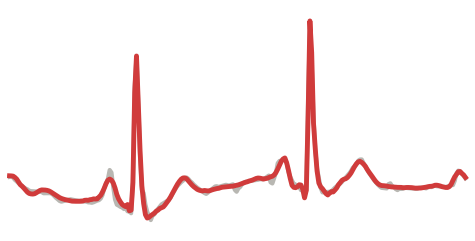
\includegraphics[width=2.3cm]{../figures/cae_out.png}};
  \node[lbl, below=1mm of out] {реконструкция \(\hat{x}\)\\\(1 \times 256\)};
  \draw[arr] (d4) -- node[lbl, above, font=\tiny] {Conv1d} (out);

  % ---------------- groups ----------------
  \draw[encC!60, dashed, rounded corners=3pt] (1.45,-2.6) rectangle (6.6,1.75);
  \node[font=\small, text=encC] (ico1) at (1.9,2.05) {\faMicrochip};
  \node[lbl, anchor=west, text=encC!60!black] at (ico1.east) {\textbf{Енкодер}: ESP32-S3, 78\,560 параметъра};
  \node[lbl, text=encC!60!black, font=\tiny] at (4.05,-2.15) {3 \(\times\) [Conv1d \(k{=}5\), стъпка 2, ReLU]\\\(\rightarrow\) Flatten \(\rightarrow\) Linear};

  \draw[decC!60, dashed, rounded corners=3pt] (9.85,-2.6) rectangle (16.1,1.75);
  \node[font=\small, text=decC] (ico2) at (10.3,2.05) {\faDesktop};
  \node[lbl, anchor=west, text=decC!60!black] at (ico2.east) {\textbf{Декодер}: компютър, 81\,809 параметъра};
  \node[lbl, text=decC!60!black, font=\tiny] at (12.95,-2.15) {Linear \(\rightarrow\) 3 \(\times\) [Upsample \(\times 2\),\\Conv1d \(k{=}5\), ReLU] \(\rightarrow\) Conv1d};
\end{tikzpicture}
}
    \caption{Архитектура на финалния едномерен конволюционен автоенкодер (ширина 16, \(d = 32\)). Блоковете показват междинните тензори (канали \(\times\) дължина): синьо -- енкодер, изпълняван на ESP32-S3; оранжево -- декодер, изпълняван на компютъра; зелено -- латентният вектор, предаван като 32 байта int8. Сигналите вляво и вдясно са реален тестов прозорец и неговата реконструкция.}
    \label{fig:cae}
\end{figure}

Декодерът е огледален: линеен слой възстановява тензор \(64 \times 32\), след което три стъпала от линейно увеличаване на дължината (upsampling) и конволюция възстановяват 256 отчета, а последна конволюция дава един изходен канал. Вместо транспонирани конволюции е използвано увеличаване на дължината с последваща конволюция, което избягва артефактите от типа \enquote{шахматна дъска}. Енкодерът съдържа само конволюции, ReLU и линеен слой -- операции, които се реализират директно на микроконтролер. Нормализиращи слоеве, механизми за внимание и други операции, трудни за вградено изпълнение, не са използвани.

\subsection{Обучение}
Моделът е реализиран на \texttt{PyTorch} \cite{paszke2019pytorch} и се обучава чрез минимизиране на средноквадратичната грешка с оптимизатора \texttt{Adam} \cite{kingma2015adam}. Скоростта на обучение се намалява наполовина, когато валидационната грешка не се подобри в продължение на 5 епохи, а обучението спира, когато няма подобрение в продължение на 15 епохи. Запазва се моделът с най-ниска валидационна грешка. PRD и PRDN се използват като показатели за оценка, а не като функция на загубата. Хиперпараметрите са обобщени в \cref{tab:hyper}.

\begin{table}[htbp]
    \centering
    \begin{tabular}{l l}
        \toprule
        Параметър & Стойност \\
        \midrule
        Функция на загубата & средноквадратична грешка (MSE) \\
        Оптимизатор & Adam, начална скорост \(10^{-3}\) \\
        Размер на пакета & 128 прозореца \\
        Намаляване на скоростта & \(\times 0.5\) при 5 епохи без подобрение, минимум \(10^{-5}\) \\
        Ранно спиране & 15 епохи без подобрение, максимум 150 епохи \\
        Начално състояние на генератора & 42 \\
        \bottomrule
    \end{tabular}
    \caption{Хиперпараметри на обучението.}
    \label{tab:hyper}
\end{table}

\subsection{Програмна реализация}
Кодът е организиран като Python пакет с отделни модули за зареждане на данните, филтрация, прозорци, модел, обучение, оценка, квантуване и фигури. Всеки експеримент се описва с YAML конфигурация, а средата е заключена с пакетния мениджър \texttt{pixi} \cite{pixi} за възпроизводимост. Обучението е проведено на NVIDIA GeForce RTX 4060 (Laptop GPU) и отнема 2--8 s на епоха в зависимост от ширината на модела. Основните функции са покрити с автоматични тестове.

% =====================================================================
\section{Експерименти и резултати}
Всички резултати в този раздел са получени върху тестовия дял (дял 10), който не е използван нито за обучение, нито за избор на модел. За всяка конфигурация се отчитат медианата, интерквартилният диапазон (IQR) и средната стойност на PRDN по прозорци. Медианата на ниво запис се различава от медианата по прозорци с по-малко от 1 процентен пункт във всички експерименти, поради което в таблиците е дадена само втората.

\subsection{Капацитет на модела}
Първият въпрос беше дали началният модел е ограничен от капацитета си. При \(d = 16\) бяха сравнени три ширини на енкодера и декодера (\cref{tab:width}). Удължаването на обучението на тесния модел (ширина 8) от 50 на 150 епохи подобри медианата на PRDN само от 33.5\% на 33.3\%, което показва, че моделът е ограничен от капацитета, а не от продължителността на обучението. Удвояването на ширината до 16 намали медианата до 28.9\%. По-нататъшното удвояване до 32 подобри резултата само с 0.3 процентни пункта, утрои времето за епоха и увеличи разликата между обучаващата и валидационната грешка от 6\% на 20\%, което е признак за начало на преобучаване. Затова за всички следващи експерименти е избрана ширина 16.

\begin{table}[htbp]
    \centering
    \begin{tabular}{l r r c c}
        \toprule
        Ширина (канали) & Енкодер & Декодер & MSE обуч./вал. & PRDN медиана (IQR) \\
        \midrule
        8 (\(8 \rightarrow 16 \rightarrow 32\)) & 19\,696 & 21\,001 & 0.128 / 0.125 & 33.3\% (24.9--45.3) \\
        16 (\(16 \rightarrow 32 \rightarrow 64\)) & 45\,776 & 49\,041 & 0.090 / 0.095 & 28.9\% (21.6--39.7) \\
        32 (\(32 \rightarrow 64 \rightarrow 128\)) & 117\,136 & 126\,241 & 0.079 / 0.095 & 28.6\% (21.0--39.2) \\
        \bottomrule
    \end{tabular}
    \caption{Влияние на ширината на модела при \(d = 16\) (брой параметри, MSE в нормализирани единици и PRDN на тестовия дял).}
    \label{tab:width}
\end{table}

\subsection{Размер на латентния вектор}
Основният експеримент изследва размера на латентния вектор при фиксирана ширина 16. \Cref{fig:sweep} и \cref{tab:sweep} показват резултатите за \(d = 8, 16, 32\), което съответства на степени на компресия 64:1, 32:1 и 16:1 при int8 латентен вектор. Качеството на реконструкцията се подобрява плавно с увеличаване на \(d\): всяко удвояване на латентния вектор намалява медианата на PRDN приблизително с 37\% (от 45.4\% на 28.9\% и след това на 17.9\%). В рамките на изследвания диапазон не се наблюдава насищане. При \(d = 32\) 60\% от тестовите прозорци имат PRDN под 20\%, а 4.2\% са под границата от 9\%, докато при \(d = 16\) тези дялове са съответно 19\% и 0\%.

\begin{figure}[htbp]
    \centering
    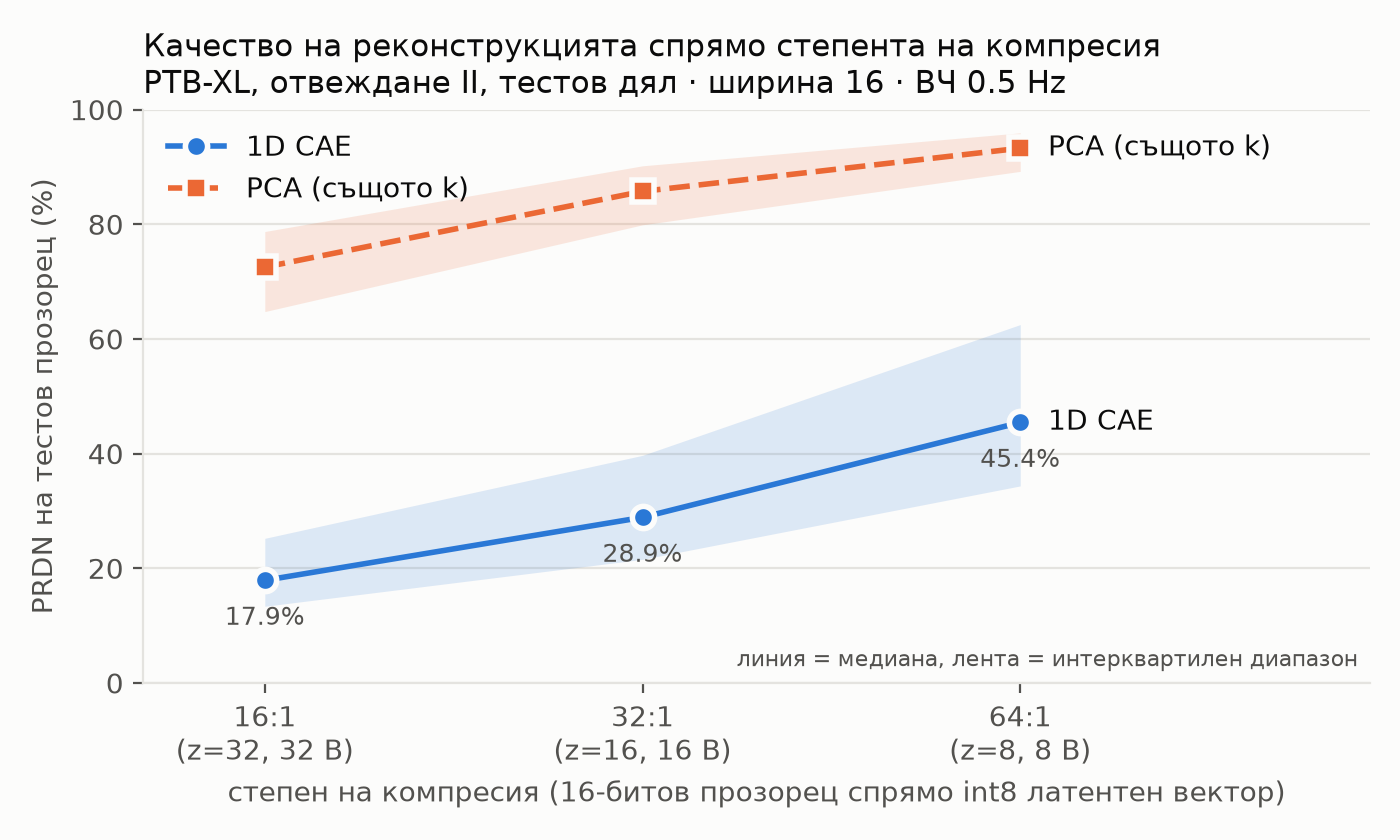
\includegraphics[width=0.78\textwidth]{../figures/latent_sweep.png}
    \caption{PRDN на тестовите прозорци в зависимост от степента на компресия за 1D CAE и PCA със същия брой компоненти. Линията показва медианата, а лентата -- интерквартилния диапазон.}
    \label{fig:sweep}
\end{figure}

\begin{table}[htbp]
    \centering
    \begin{tabular}{c c c r c c c}
        \toprule
        \(d\) & Обем & CR & Енкодер & CAE, float \(z\) & CAE, int8 \(z\) & PCA \\
        \midrule
        8 & 8 B & 64:1 & 29\,384 & 45.4\% (34.4--62.5) & 46.6\% & 93.3\% \\
        16 & 16 B & 32:1 & 45\,776 & 28.9\% (21.6--39.7) & 29.3\% & 85.7\% \\
        32 & 32 B & 16:1 & 78\,560 & 17.9\% (13.4--25.2) & 18.2\% & 72.5\% \\
        \bottomrule
    \end{tabular}
    \caption{Медиана (IQR) на PRDN на тестовия дял в зависимост от размера на латентния вектор (ширина 16, филтрация с нулева фаза).}
    \label{tab:sweep}
\end{table}

Автоенкодерът превъзхожда PCA с 3.3 до 4 пъти при всяка степен на компресия. PCA с 16 компоненти обяснява само 32\% от дисперсията на прозорците, тъй като сърдечните удари попадат на различни позиции в прозореца и линейната база не може да опише това отместване. Дори при 64:1 автоенкодерът (45\%) е по-добър от PCA при 16:1 (73\%). Това е основният аргумент за използване на нелинеен модел.

\Cref{fig:recon_by_z} показва едни и същи тестови прозорци, реконструирани с трите модела. При \(d = 8\) моделът възстановява позициите и приблизителната амплитуда на QRS комплексите, но изглажда P и T вълните. При \(d = 32\) формата на P, QRS и T е възстановена добре при прозорците с регулярен ритъм. Трудните прозорци съдържат учестен или неравномерен ритъм с много удари и ниска амплитуда, при които латентният вектор не е достатъчен, за да кодира позицията и формата на всеки удар.

\begin{figure}[htbp]
    \centering
    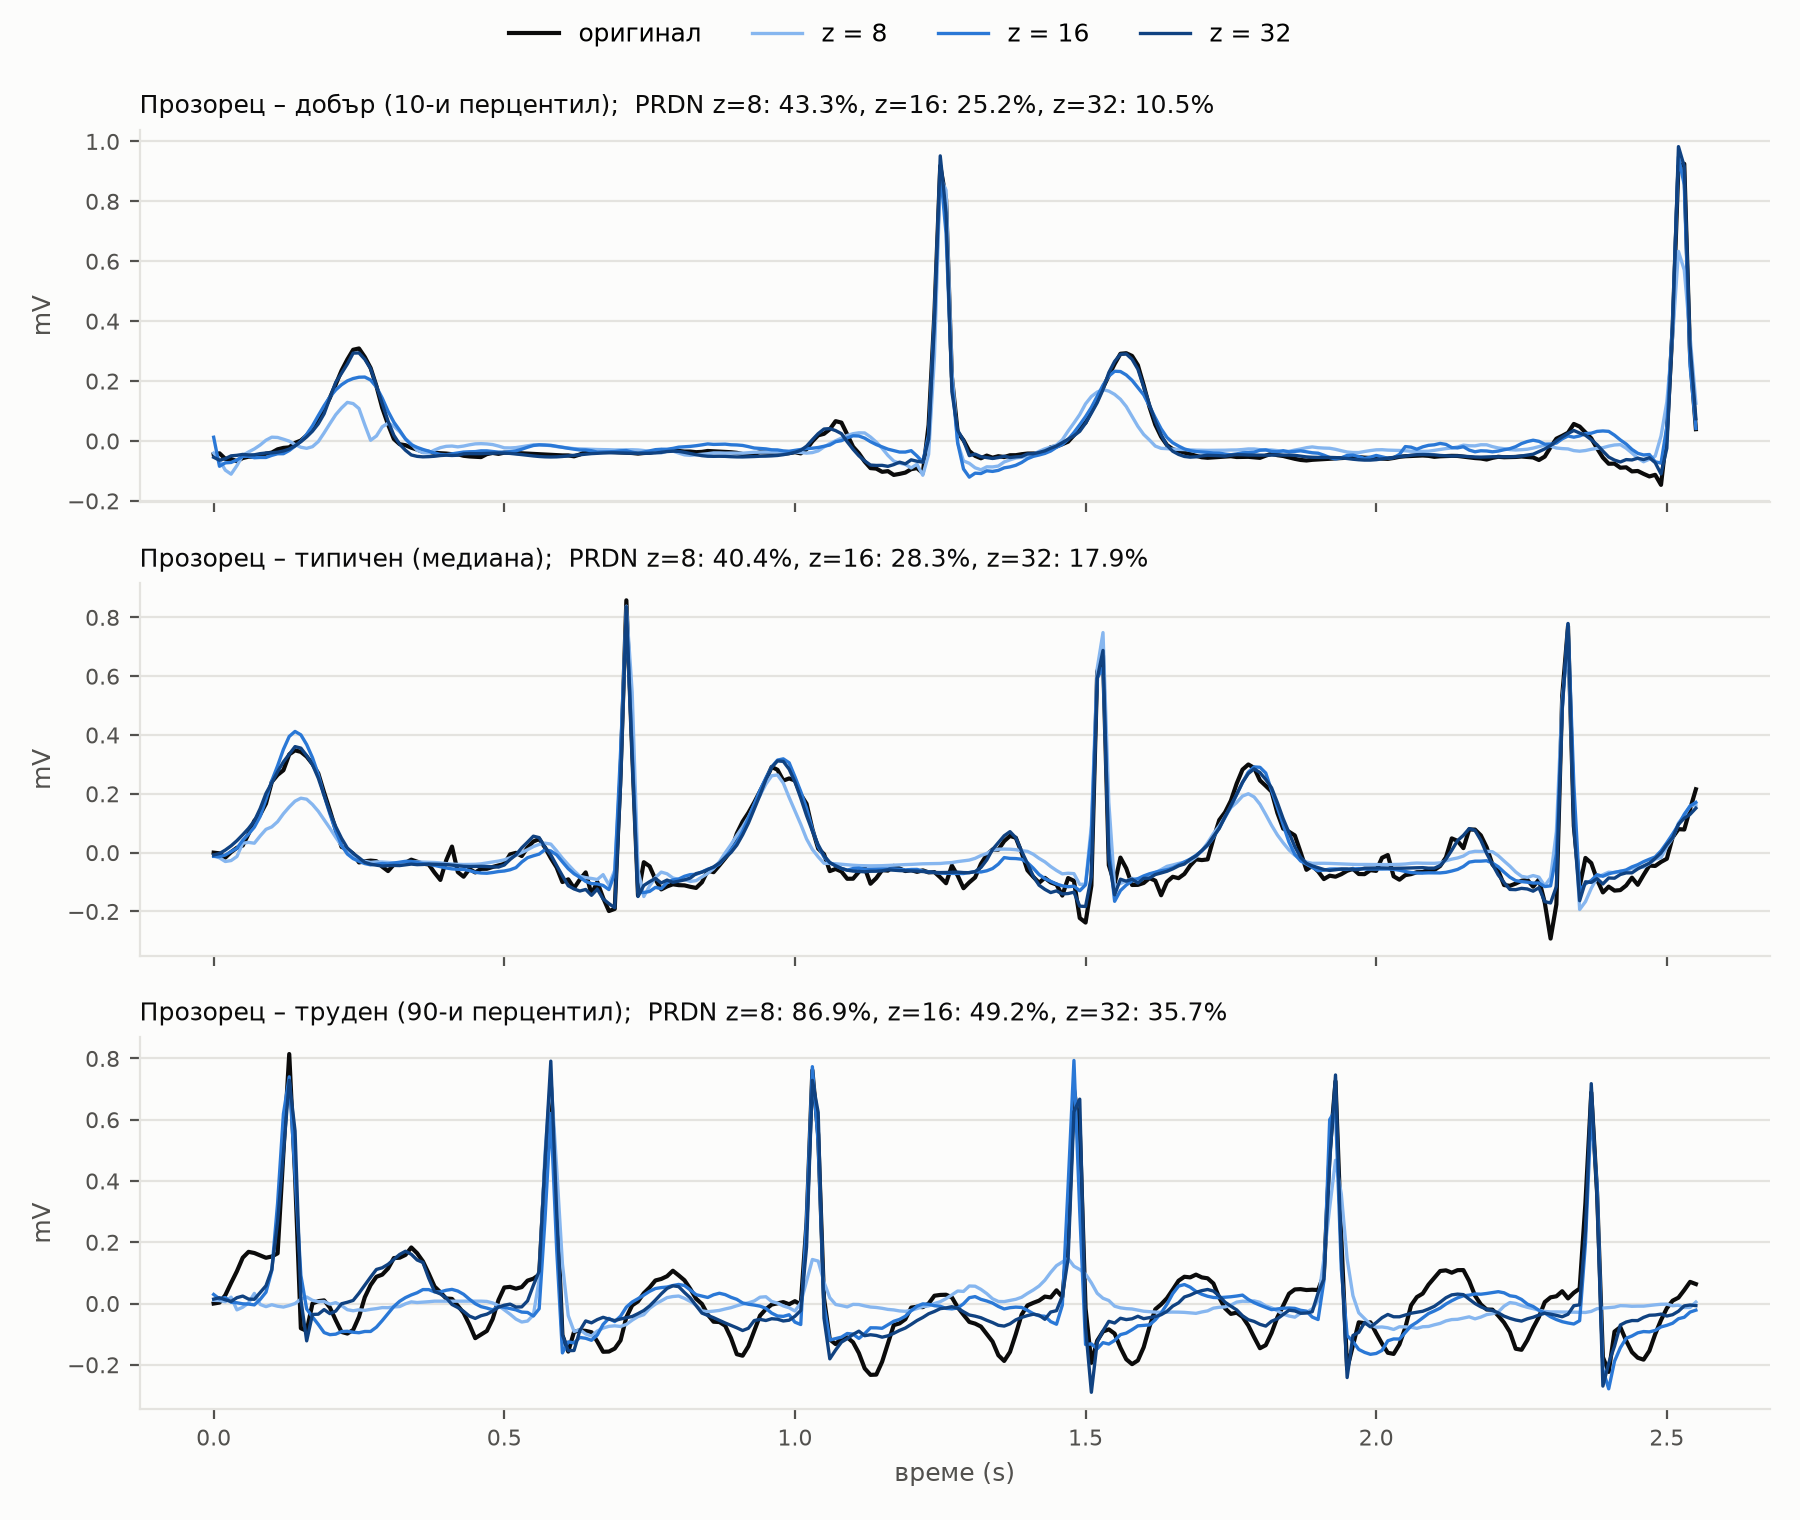
\includegraphics[width=0.86\textwidth]{../figures/recon_by_z.png}
    \caption{Едни и същи тестови прозорци, реконструирани с \(d = 8\), 16 и 32. Прозорците са избрани по PRDN на модела с \(d = 32\) (10-и, 50-и и 90-и перцентил).}
    \label{fig:recon_by_z}
\end{figure}

И трите модела се сближават стабилно: моделите с \(d = 8\) и \(d = 16\) спират след 127 и 126 епохи поради липса на подобрение, а моделът с \(d = 32\) достига ограничението от 150 епохи с минимална скорост на обучение, което предполага, че по-дълго обучение би дало малко допълнително подобрение.

\subsection{Квантуване на латентния вектор}
Степените на компресия в \cref{tab:sweep} предполагат, че латентният вектор се предава като 8-битови цели числа. Това беше проверено чрез квантуване след обучението (post-training quantization) само на латентния вектор, без промяна на модела. За всяка латентна координата се определят долна граница \(l_j\) и стъпка \(\Delta_j\) от 0.1-ви и 99.9-и перцентил на стойностите ѝ в обучаващия дял:
\begin{equation}
    q_j = \operatorname{clip}\!\left(\operatorname{round}\!\left(\frac{z_j - l_j}{\Delta_j}\right), 0, 255\right) - 128,
    \qquad
    \hat{z}_j = (q_j + 128)\,\Delta_j + l_j .
    \label{eq:quant}
\end{equation}
Параметрите \(l_j\) и \(\Delta_j\) са константи, известни на енкодера и декодера, и не се предават с всеки прозорец. Квантуването увеличава медианата на PRDN с 0.4 процентни пункта при \(d = 16\) и с 0.3 процентни пункта при \(d = 32\) (\cref{tab:sweep}), а извън обхвата попадат около 0.15\% от латентните стойности. Следователно степените на компресия 32:1 и 16:1 са потвърдени експериментално с пренебрежима загуба на качество.

\subsection{Каузална филтрация}
\label{sec:causal}
Всички модели дотук са обучени върху данни, филтрирани с нулева фаза, докато устройството може да използва само каузален филтър. Затова моделът с \(d = 32\) беше обучен повторно върху каузално филтрирани данни, а резултатите са обобщени в \cref{tab:causal}.

\begin{table}[htbp]
    \centering
    \begin{tabular}{l c}
        \toprule
        Сравнение (тестов дял, \(d = 32\)) & PRDN медиана \\
        \midrule
        Модел с нулева фаза, вход и референция с нулева фаза & 17.9\% \\
        Каузален модел, вход и референция с каузален филтър & 18.3\% (int8: 18.7\%) \\
        Модел с нулева фаза, подаден каузален вход & 21.3\% \\
        Каузално спрямо филтрирано с нулева фаза (само филтър) & 25.8\% \\
        Каузален модел спрямо референция с нулева фаза & 32.8\% \\
        \bottomrule
    \end{tabular}
    \caption{Влияние на каузалната филтрация върху качеството на реконструкцията.}
    \label{tab:causal}
\end{table}

Резултатите водят до три извода. Първо, каузално филтрираният сигнал се компресира почти толкова добре, колкото филтрираният с нулева фаза (18.3\% срещу 17.9\%). Второ, моделът трябва да бъде обучен със същия филтър, който ще се използва в устройството: подаването на каузален вход на модела, обучен с нулева фаза, увеличава грешката до 21.3\%. Трето, самият каузален филтър от 0.5 Hz променя формата на сигнала повече от компресията: разликата между двата филтрирани сигнала е 25.8\% PRDN, като част от нея се дължи на различната амплитудна характеристика (двукратното прилагане при \texttt{sosfiltfilt}), а част е реално фазово изкривяване на ST сегмента (\cref{fig:filter_example}). Следователно в предложения апарат основният източник на изкривяване е предварителната обработка, а не компресията.

\subsection{Финален модел}
За крайна конфигурация на апарата е избран моделът с \(d = 32\), ширина 16 и каузален високочестотен филтър от 0.5 Hz. Той постига медиана на PRDN 18.3\% (IQR 13.7--25.7\%) с float латентен вектор и 18.7\% с int8 латентен вектор при степен на компресия 16:1. Изборът на \(d = 32\) пред \(d = 16\) се обосновава с това, че при едноканален ЕКГ със 100 Hz суровият поток е само 200 B/s и разликата между 12.5 B/s и 6.25 B/s е пренебрежима за всяка безжична връзка, докато разликата в качеството е 10.6 процентни пункта. \Cref{fig:final_examples} показва най-добрите, типичните и най-лошите реконструкции на финалния модел в сравнение с PCA.

\begin{figure}[htbp]
    \centering
    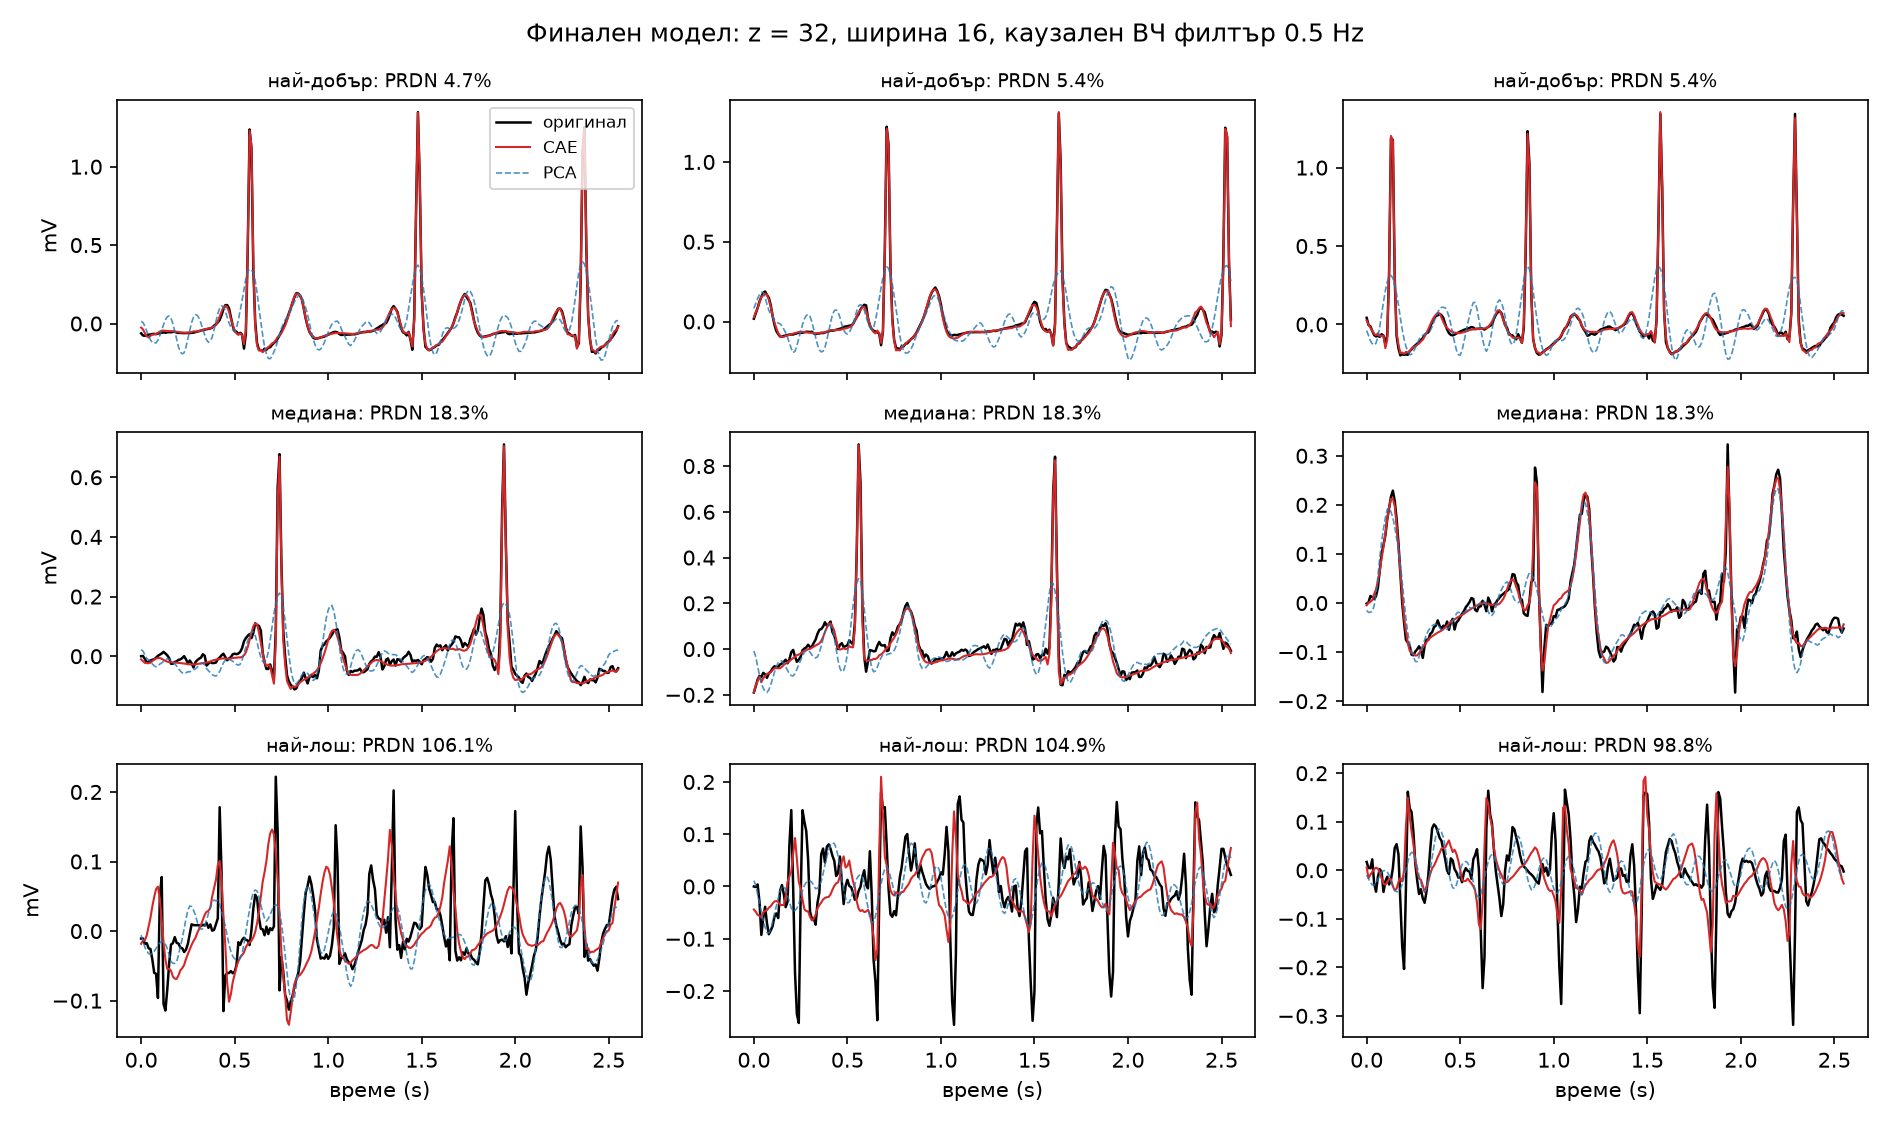
\includegraphics[width=0.94\textwidth]{../figures/final_examples.png}
    \caption{Най-добри, медианни и най-лоши тестови прозорци на финалния модел (червено) в сравнение с PCA с 32 компоненти (пунктир) и оригиналния сигнал (черно).}
    \label{fig:final_examples}
\end{figure}

Анализът на грешките по анотациите за качество в PTB-XL показва, че статичният шум и импулсните смущения увеличават грешката само с 2--4 процентни пункта, докато основната причина за най-лошите реконструкции е ритъмът: учестени или неравномерни ритми с ниска амплитуда, при които в един прозорец попадат 5--7 удара.

% =====================================================================
\section{Концепция за интеграция в апарат}
Основният фокус на проекта е алгоритъмът за компресия. Този раздел представя концепция за това как обученият автоенкодер може да бъде вграден в реална инженерна система: кои компоненти са избрани, как се свързват и коя част от алгоритъма се изпълнява на всеки от тях. Разделът не е подробен електрически проект. Свързването на такава схема към човек изисква изолация и съответствие с IEC 60601-1 \cite{iec60601}, поради което предложеният апарат се захранва от батерия и предава данните безжично.

\subsection{Избрани компоненти}
Системата се състои от три части: аналогов преден блок, който регистрира ЕКГ, микроконтролер, който изпълнява енкодера, и компютър, който изпълнява декодера.

\begin{description}
    \item[ADS1292R (Texas Instruments)] двуканален аналогов преден блок за ЕКГ с 24-битови делта-сигма АЦП, програмируем усилвател, RLD усилвател, детекция на откачен електрод, вградено опорно напрежение и SPI интерфейс \cite{ti_ads1292r}. Консумацията от 335 \(\mu\)W на канал и CMRR от 120 dB го правят подходящ за преносим апарат.
    \item[ESP32-S3 (Espressif)] микроконтролер с два ядра Xtensa LX7 до 240 MHz, хардуерни операции с плаваща запетая, векторни инструкции за невронни мрежи, 512 KB SRAM, външна флаш памет и PSRAM, Wi-Fi и Bluetooth 5 (LE) \cite{espressif_esp32s3}. Препоръчва се модул с PSRAM, например ESP32-S3-WROOM-1-N8R8.
    \item[Компютър] приема латентните вектори, възстановява сигнала с декодера и го визуализира или съхранява.
\end{description}

Функционалната блокова схема на ADS1292R е показана на \cref{fig:ads_block}. В проекта се използва само втората верига на канал: входният мултиплексор (MUX) подава отвеждане II към усилвателя A2 и преобразувателя ADC2, RLD усилвателят задвижва електрода RL, а резултатите се четат през SPI интерфейса. Каналът с модулатора и демодулатора за дишане (RESP MOD, RESP DEMOD, ADC1) не е необходим за ЕКГ и остава неизползван. Най-ниската честота на дискретизация на ADS1292R е 125 SPS, затова апаратът дискретизира с 500 SPS и микроконтролерът намалява честотата до 100 Hz, както е описано в \cref{sec:data}. Пълните технически спецификации на двата основни компонента са дадени в края на документа.

\begin{figure}[htbp]
    \centering
    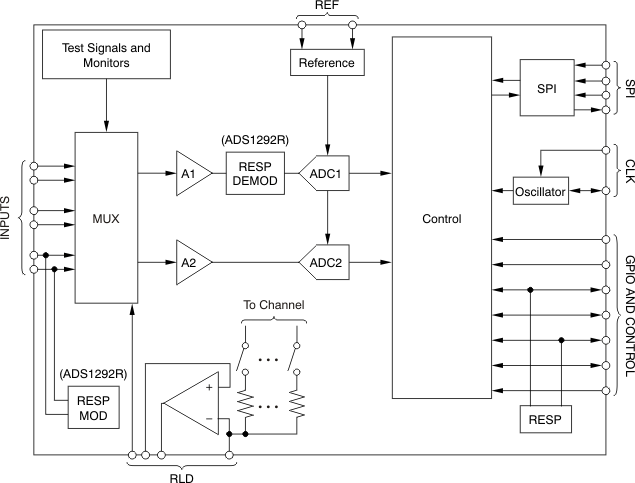
\includegraphics[width=0.66\textwidth]{ads1292r_block.png}
    \caption{Функционална блокова схема на ADS1292R. В проекта се използват входният мултиплексор, усилвателят A2, ADC2, RLD усилвателят, опорното напрежение и SPI интерфейсът. Фигурата е взета от продуктовата страница на Texas Instruments \cite{ti_ads1292r}.}
    \label{fig:ads_block}
\end{figure}

\subsection{Свързване на компонентите}
Свързването на компонентите е показано на \cref{fig:connection}. Електродите на левия крак и дясната ръка се подават на диференциалния вход на канал 2 (IN2P и IN2N), което дава отвеждане II, а електродът на десния крак се задвижва от изхода RLDOUT. ADS1292R и ESP32-S3 са свързани по SPI шина (SCLK, DIN, DOUT, CS) и две управляващи линии: START стартира преобразуването, а DRDY сигнализира за всеки нов отчет и предизвиква прекъсване в микроконтролера. Предложените изводи на ESP32-S3 съвпадат с хардуерните изводи на неговия SPI интерфейс. Микроконтролерът изпраща квантуваните латентни вектори безжично към компютъра. Двата чипа се захранват от общо напрежение 3.3 V от литиево-полимерна батерия през линеен стабилизатор.

\begin{figure}[htbp]
    \centering
    \resizebox{\textwidth}{!}{% Simplified connection of the selected parts: electrodes -> ADS1292R -> SPI -> ESP32-S3 -> radio -> PC.
% Pin names sit just inside the chip edges; wires run between the chip edges.
\begin{tikzpicture}[
    font=\footnotesize,
    chip/.style={draw, very thick, fill=gray!6},
    el/.style={circle, draw, thick, minimum size=8mm, fill=white, font=\scriptsize},
    pin/.style={font=\scriptsize\ttfamily},
    to/.style={thick, -{Stealth[length=2mm]}},
  ]
  % ---- ADS1292R: x 2.5 .. 7.5
  \draw[chip] (2.5,-0.1) rectangle (7.5,4.4);
  \node[font=\footnotesize\bfseries, anchor=north] at (5.0,4.35) {ADS1292R};
  \node[align=center, font=\scriptsize] at (5.0,1.9) {канал 2:\\PGA (\(G = 6\))\\\(\Delta\Sigma\) АЦП, 24 bit\\500 SPS\\[2pt]RLD усилвател};

  % ---- ESP32-S3: x 10.0 .. 15.0
  \draw[chip] (10.0,-0.1) rectangle (15.0,4.4);
  \node[font=\footnotesize\bfseries, anchor=north] at (12.5,4.35) {ESP32-S3};
  \node[align=center, font=\scriptsize] at (13.05,1.9) {децимация 5:1\\ВЧ филтър 0.5 Hz\\буфер 256 отчета\\[2pt]\textbf{CAE енкодер}\\квантуване на \(z\) до int8};

  % ---- PC
  \node[draw, thick, rounded corners=2pt, align=center, fill=white, text width=2.4cm, minimum height=2.4cm] (pc) at (18.2,2.15)
    {Компютър\\[3pt]деквантуване\\\textbf{CAE}\\\textbf{декодер}\\визуализация};

  % ---- electrodes -> analog inputs
  \node[el] (LL) at (0.2,3.3) {LL};
  \node[el] (RA) at (0.2,2.1) {RA};
  \node[el] (RL) at (0.2,0.6) {RL};
  \node[pin, anchor=west] at (2.55,3.3) {IN2P};
  \node[pin, anchor=west] at (2.55,2.1) {IN2N};
  \node[pin, anchor=west] at (2.55,0.6) {RLDOUT};
  \draw[to] (LL.east) -- (2.5,3.3);
  \draw[to] (RA.east) -- (2.5,2.1);
  \draw[to] (2.5,0.6) -- (RL.east);
  \node[font=\scriptsize] at (1.35,3.95) {отвеждане II};
  \node[font=\scriptsize] at (1.1,-0.2) {активна референция};

  % ---- SPI and control: ESP32-S3 -> ADS1292R
  \foreach \sig/\gpio/\y in {SCLK/GPIO12/3.7, DIN/GPIO11/3.1, CS/GPIO10/1.9, START/GPIO14/0.7}{
    \node[pin, anchor=east] at (7.45,\y) {\sig};
    \node[pin, anchor=west] at (10.05,\y) {\gpio};
    \draw[to] (10.0,\y) -- (7.5,\y);
  }
  % ---- ADS1292R -> ESP32-S3 (data, data-ready interrupt)
  \foreach \sig/\gpio/\y in {DOUT/GPIO13/2.5, DRDY/GPIO9/1.3}{
    \node[pin, anchor=east] at (7.45,\y) {\sig};
    \node[pin, anchor=west] at (10.05,\y) {\gpio};
    \draw[to] (7.5,\y) -- (10.0,\y);
  }
  \node[font=\scriptsize] at (8.75,4.7) {SPI + управление};

  % ---- radio link
  \draw[to] (15.0,2.15) -- node[above, font=\scriptsize] {BLE / Wi-Fi} node[below, font=\scriptsize, align=center] {32 B на\\2.56 s} (pc.west);

  % ---- power
  \node[font=\scriptsize, text=gray!50!black, anchor=north] at (8.75,-0.3) {общо захранване 3.3 V от Li-Po батерия през линеен стабилизатор (LDO)};
\end{tikzpicture}
}
    \caption{Свързване на избраните компоненти: електроди, ADS1292R, ESP32-S3 и компютър. Стрелките показват посоката на сигналите, а изводите на ESP32-S3 са предложение.}
    \label{fig:connection}
\end{figure}

\subsection{Връзка между автоенкодера и апарата}
\Cref{fig:system} показва как разработеният алгоритъм се разпределя между компонентите. Обучението се извършва веднъж на компютър. След него във флаш паметта на ESP32-S3 се записват теглата на енкодера и константите на предварителната обработка (коефициентите на филтъра, мащабът \(s\) и параметрите за квантуване \(l_j, \Delta_j\)), а теглата на декодера остават на компютъра.

\begin{figure}[htbp]
    \centering
    \resizebox{\textwidth}{!}{% How the trained CAE is split between the device and the computer (simplified).
% Top: training happens once, offline. Bottom: the live signal path.
\begin{tikzpicture}[
  font=\footnotesize,
  >={Stealth[length=1.8mm]},
  arr/.style={->, thick, black!70},
  dep/.style={->, thick, dashed, black!45},
  lbl/.style={font=\scriptsize, text=black!75, align=center},
  box/.style={draw=#1!80!black, fill=#1!12, line width=0.6pt, rounded corners=3pt,
              align=center, minimum height=1.5cm, text width=3.1cm},
  thumb/.style={inner sep=0pt}]

  \colorlet{encC}{blue!55!cyan}
  \colorlet{decC}{orange!85!red}
  \colorlet{latC}{green!50!black}
  \colorlet{offC}{black!60}

  % ---------------- live signal path ----------------
  \node[box=offC, text width=2.7cm] (ads) at (0,0) {\textbf{ADS1292R}\\[2pt]отвеждане II\\500 SPS, 24 bit};
  \node[box=encC] (esp) at (4.5,0) {\textbf{ESP32-S3}\\[2pt]ВЧ филтър\\прозорец 256\\\textbf{енкодер} \(\rightarrow z\)};
  \node[box=decC] (pc) at (10.0,0) {\textbf{Компютър}\\[2pt]\textbf{декодер}\\\(z \rightarrow \hat{x}\)};
  \node[thumb] (out) at (13.6,0) {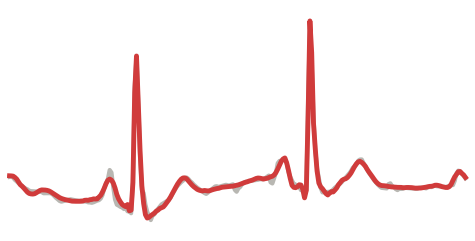
\includegraphics[width=2.2cm]{../figures/cae_out.png}};
  \node[lbl, below=1mm of out] {реконструиран ЕКГ};

  \node[font=\small, text=encC] at ($(esp.north east)+(-0.3,-0.3)$) {\faMicrochip};
  \node[font=\small, text=decC] at ($(pc.north east)+(-0.3,-0.3)$) {\faDesktop};

  \draw[arr] (ads) -- node[lbl, above] {SPI} (esp);
  \draw[->, thick, latC] (esp) -- node[lbl, above, text=latC!60!black] {32 B int8} node[lbl, below, text=latC!60!black] {на всеки 2.56 s} (pc);
  \draw[arr] (pc) -- (out);

  % ---------------- training, once ----------------
  \node[box=offC, fill=black!4, text width=4.2cm, minimum height=1.1cm] (train) at (7.15,2.9)
    {\textbf{Обучение на CAE} (веднъж, офлайн)\\PTB-XL, PyTorch, GPU};
  \draw[dep] (train.south) -- ++(0,-0.45) -| node[lbl, pos=0.75, left] {тегла на енкодера,\\филтър, мащаб, int8} (esp.north);
  \draw[dep] (train.south) -- ++(0,-0.45) -| node[lbl, pos=0.75, right] {тегла на\\декодера} (pc.north);
\end{tikzpicture}
}
    \caption{Разпределение на обучения автоенкодер в апарата: енкодерът работи на ESP32-S3, декодерът -- на компютъра, а между тях се предават 32 байта на всеки прозорец.}
    \label{fig:system}
\end{figure}

По време на работа ESP32-S3 повтаря стъпките от предварителната обработка в Python, но в каузален вариант: на всеки отчет от ADS1292R прилага нискочестотен филтър и децимация 5:1, после каузалния високочестотен филтър, и натрупва отчетите в буфер. На всеки 256 нови отчета (2.56 s) прозорецът се мащабира, подава се на енкодера, а латентният вектор от 32 числа се квантува до int8 и се изпраща като 32 байта. Компютърът деквантува вектора, възстановява прозореца с декодера и долепя последователните прозорци в непрекъснат сигнал. Правилността на вградената реализация може да се провери с еталонни вектори: прозорци от тестовия дял заедно с латентните вектори, изчислени в Python.

\Cref{tab:budget} показва, че енкодерът е подходящ за ESP32-S3. Той изисква около 567 хиляди операции умножение-събиране на прозорец, което по оценка съответства на 5--15 ms при 240 MHz, докато нов прозорец постъпва на всеки 2.56 s. Теглата в float32 заемат около 307 KiB флаш памет, а междинните буфери са под 20 KiB. Следователно енкодерът може да работи без квантуване на теглата. Квантуването на теглата до int8 чрез ESP-DL \cite{espdl} би намалило паметта и времето около 4 пъти, но не е необходимо.

\begin{table}[htbp]
    \centering
    \begin{tabular}{l r l}
        \toprule
        Ресурс & Стойност & Наличен ресурс \\
        \midrule
        Параметри на енкодера & 78\,560 & -- \\
        Тегла (float32) & 307 KiB & флаш (8 MB) \\
        Междинни буфери & \(\approx\)16 KiB & 512 KB SRAM \\
        Умножения-събирания на прозорец & \(\approx\)567\,000 & -- \\
        Оценено време за изпълнение & 5--15 ms & 2\,560 ms между прозорците \\
        Поток след децимация (16 bit, 100 Hz) & 200 B/s & -- \\
        Поток на латентните вектори & 12.5 B/s & BLE или Wi-Fi \\
        \bottomrule
    \end{tabular}
    \caption{Оценени ресурси за изпълнение на енкодера на ESP32-S3 и потоци от данни. Времето за изпълнение е оценка и трябва да бъде измерено върху реалния модул.}
    \label{tab:budget}
\end{table}

% =====================================================================
\section{Обсъждане}
Най-важният резултат от проекта е, че размерът на латентния вектор определя плавен компромис между степента на компресия и качеството: всяко удвояване на \(d\) намалява медианата на PRDN приблизително с 37\%, без насищане в изследвания диапазон. Капацитетът на мрежата има по-малко значение: след ширина 16 моделът започва да се преобучава, а качеството почти не се подобрява. Следователно ограничението на системата е основно в латентния вектор, а не в конволюционните слоеве. Нелинейният автоенкодер е 3--4 пъти по-добър от PCA при еднакъв обем на данните, което потвърждава ползата от невронна мрежа за тази задача.

Постигнатото качество не е достатъчно за клинично приложение. Медианата от 18.7\% PRDN е над границата от 9\%, която се свързва с добро качество при компресия на ЕКГ \cite{zigel2000wdd}, макар част от прозорците с регулярен ритъм да я достигат. Освен това 100-херцовата дискретизация ограничава честотната лента до 50 Hz, което е под препоръчаните 150 Hz за диагностична ЕКГ при възрастни \cite{kligfield2007aha}. Проектът демонстрира принципа на компресия в устройството, но не заменя диагностичен електрокардиограф.

Анализът на каузалната филтрация показа, че изкривяването от предварителната обработка може да бъде по-голямо от изкривяването от компресията. За реален апарат се препоръчва линейно-фазов FIR високочестотен филтър, който запазва формата на вълните с цената на фиксирано закъснение от 1--3 s (приемливо, тъй като устройството и без това буферира 2.56-секундни прозорци), или каузален филтър с гранична честота 0.05 Hz, съобразен с препоръката на AHA.

Други ограничения са, че показателите са изчислени върху сигнали от PTB-XL, а не от ADS1292R, и сигналът от реалния апарат може да се различава по шум и характеристики на електродите. Времето за изпълнение на енкодера на ESP32-S3 е оценено, а не измерено. Като бъдеща работа могат да се разгледат: реализация на енкодера на C и проверка с еталонни вектори, измерване на времето и консумацията върху модул ESP32-S3, линейно-фазов FIR филтър, по-големи латентни вектори и прозорци, както и функции на загубата, които наказват по-силно грешките в QRS комплекса.

% =====================================================================
\section{Заключение}
В курсовия проект е проектиран концептуален едноканален електрокардиографски апарат на базата на ADS1292R и ESP32-S3 и е разработен алгоритъм за компресия на ЕКГ сигнала чрез едномерен конволюционен автоенкодер. Алгоритъмът е обучен и оценен върху PTB-XL при строго разделяне на данните по пациенти, а качеството е измерено чрез PRD и PRDN.

Експериментите показаха, че ширина 16 е най-подходящият капацитет на модела, а размерът на латентния вектор определя компромиса между качество и компресия: медианата на PRDN е 45.4\%, 28.9\% и 17.9\% при степени на компресия 64:1, 32:1 и 16:1. Квантуването на латентния вектор до int8 струва под половин процентен пункт при \(d \ge 16\), а моделът, обучен с каузален филтър, постига 18.7\% PRDN при условия, съответстващи на реалния апарат. Енкодерът с около 79 хиляди параметъра може да бъде изпълнен в реално време на ESP32-S3 без квантуване на теглата.

Концепцията за интеграция показва как алгоритъмът се вгражда в инженерна система: ADS1292R регистрира отвеждане II, ESP32-S3 изпълнява предварителната обработка и енкодера, а компютърът възстановява сигнала с декодера. Резултатите са подходяща основа за реализация на прототип и за по-нататъшно изследване на компресията на биомедицински сигнали в носими устройства.

% =====================================================================
\section*{Списък с използваните означения и съкращения}
\addcontentsline{toc}{section}{Списък с използваните означения и съкращения}
\begin{spacing}{1.0}
\small
\begin{multicols}{2}
\begin{description}
    \setlength{\itemsep}{0pt}
    \item[АЦП] аналогово-цифров преобразувател
    \item[ЕКГ] електрокардиограма, електрокардиография
    \item[ВЧ / НЧ] високочестотен / нискочестотен (филтър)
    \item[AHA] American Heart Association
    \item[BLE] Bluetooth Low Energy
    \item[CAE] Convolutional Autoencoder, конволюционен автоенкодер
    \item[CMRR] Common-Mode Rejection Ratio, коефициент на потискане на синфазния сигнал
    \item[CR] Compression Ratio, степен на компресия
    \item[DRDY] Data Ready, сигнал за готов отчет на ADS1292R
    \item[FIR / IIR] филтър с крайна / безкрайна импулсна характеристика
    \item[IQR] Interquartile Range, интерквартилен диапазон
    \item[LA, RA, LL, RL] електроди на лявата ръка, дясната ръка, левия и десния крак
    \item[LDO] Low-Dropout Regulator, линеен стабилизатор с нисък пад на напрежението
    \item[MSE] Mean Squared Error, средноквадратична грешка
    \item[PCA] Principal Component Analysis, анализ на главните компоненти
    \item[PGA] Programmable Gain Amplifier, програмируем усилвател
    \item[PRD / PRDN] Percentage Root-mean-square Difference / нормиран вариант
    \item[PSRAM] Pseudo-Static RAM, външна оперативна памет
    \item[RLD] Right Leg Drive, задвижване на десния крак
    \item[SOS] Second-Order Sections, каскада от звена от втори ред
    \item[SPI] Serial Peripheral Interface, сериен периферен интерфейс
    \item[SPS] Samples Per Second, отчета в секунда
    \item[\(d\)] размерност на латентния вектор
    \item[\(f_s\)] честота на дискретизация
    \item[\(N\)] брой отчети в прозорец (256)
    \item[\(s\)] глобален мащабиращ коефициент (0.151 mV)
    \item[\(x, \hat{x}, z\)] входен прозорец, реконструкция, латентен вектор
\end{description}
\end{multicols}
\end{spacing}

% =====================================================================
\clearpage
\begin{spacing}{1.0}
\small
\begin{thebibliography}{99}
\addcontentsline{toc}{section}{Литература}

\bibitem{wagner2020ptbxl}
Patrick Wagner, Nils Strodthoff, Ralf-Dieter Bousseljot, Dieter Kreiseler, Fatima I. Lunze, Wojciech Samek and Tobias Schaeffter.
\newblock PTB-XL, a large publicly available electrocardiography dataset.
\newblock \textit{Scientific Data}, 7:154, 2020.
\newblock DOI: \url{https://doi.org/10.1038/s41597-020-0495-6}.

\bibitem{wagner2022ptbxlphysionet}
Patrick Wagner, Nils Strodthoff, Ralf-Dieter Bousseljot, Wojciech Samek and Tobias Schaeffter.
\newblock PTB-XL, a large publicly available electrocardiography dataset (version 1.0.3).
\newblock PhysioNet, 2022.
\newblock DOI: \url{https://doi.org/10.13026/kfzx-aw45}.

\bibitem{goldberger2000physionet}
Ary L. Goldberger, Luis A. N. Amaral, Leon Glass, Jeffrey M. Hausdorff, Plamen Ch. Ivanov, Roger G. Mark, Joseph E. Mietus, George B. Moody, Chung-Kang Peng and H. Eugene Stanley.
\newblock PhysioBank, PhysioToolkit, and PhysioNet: Components of a New Research Resource for Complex Physiologic Signals.
\newblock \textit{Circulation}, 101(23):e215--e220, 2000.

\bibitem{strodthoff2021deep}
Nils Strodthoff, Patrick Wagner, Tobias Schaeffter and Wojciech Samek.
\newblock Deep Learning for ECG Analysis: Benchmarks and Insights from PTB-XL.
\newblock \textit{IEEE Journal of Biomedical and Health Informatics}, 25(5):1519--1528, 2021.

\bibitem{kligfield2007aha}
Paul Kligfield, Leonard S. Gettes, James J. Bailey et al.
\newblock Recommendations for the Standardization and Interpretation of the Electrocardiogram: Part I.
\newblock \textit{Journal of the American College of Cardiology}, 49(10):1109--1127, 2007.
\newblock DOI: \url{https://doi.org/10.1016/j.jacc.2007.01.024}.

\bibitem{webster2010medical}
John G. Webster (ed.).
\newblock \textit{Medical Instrumentation: Application and Design}, 4th edition.
\newblock John Wiley \& Sons, 2010.

\bibitem{zigel2000wdd}
Yaniv Zigel, Arnon Cohen and Amos Katz.
\newblock The Weighted Diagnostic Distortion (WDD) Measure for ECG Signal Compression.
\newblock \textit{IEEE Transactions on Biomedical Engineering}, 47(11):1422--1430, 2000.

\bibitem{hinton2006reducing}
Geoffrey E. Hinton and Ruslan R. Salakhutdinov.
\newblock Reducing the Dimensionality of Data with Neural Networks.
\newblock \textit{Science}, 313(5786):504--507, 2006.

\bibitem{kingma2015adam}
Diederik P. Kingma and Jimmy Ba.
\newblock Adam: A Method for Stochastic Optimization.
\newblock \textit{International Conference on Learning Representations (ICLR)}, 2015.

\bibitem{paszke2019pytorch}
Adam Paszke et al.
\newblock PyTorch: An Imperative Style, High-Performance Deep Learning Library.
\newblock \textit{Advances in Neural Information Processing Systems 32}, 2019.

\bibitem{virtanen2020scipy}
Pauli Virtanen et al.
\newblock SciPy 1.0: Fundamental Algorithms for Scientific Computing in Python.
\newblock \textit{Nature Methods}, 17:261--272, 2020.

\bibitem{ti_ads1292r}
Texas Instruments.
\newblock ADS1292R: 2-Channel 24-Bit ADC With Integrated Respiration Impedance and ECG Front End.
\newblock \url{https://www.ti.com/product/ADS1292R}.
\newblock Accessed November 11, 2026.

\bibitem{espressif_esp32s3}
Espressif Systems.
\newblock ESP32-S3: Wi-Fi \& Bluetooth 5 (LE) SoC.
\newblock \url{https://www.espressif.com/en/products/socs/esp32-s3}.
\newblock Accessed November 11, 2026.

\bibitem{espdl}
Espressif Systems.
\newblock ESP-DL: Deep Learning Library for Espressif Chips.
\newblock GitHub repository.
\newblock \url{https://github.com/espressif/esp-dl}.

\bibitem{iec60601}
International Electrotechnical Commission.
\newblock IEC 60601-1: Medical electrical equipment -- Part 1: General requirements for basic safety and essential performance.

\bibitem{pixi}
prefix.dev.
\newblock Pixi: A Package Management Tool.
\newblock \url{https://pixi.sh}.

\end{thebibliography}
\end{spacing}

% =====================================================================
\clearpage
\section*{Технически спецификации на избраните елементи}
\addcontentsline{toc}{section}{Технически спецификации на избраните елементи}

\begin{table}[htbp]
    \centering
    \begin{tabular}{l l}
        \toprule
        Параметър & Стойност \\
        \midrule
        Брой канали & 2 (канал 1 с измерване на импеданса за дишане) \\
        АЦП & делта-сигма, 24 bit \\
        Честота на дискретизация & 125 SPS -- 8 kSPS \\
        Коефициенти на PGA & 1, 2, 3, 4, 6, 8, 12 \\
        Входен шум & 8 \(\mu\)V\textsubscript{pp} (лента 150 Hz, \(G = 6\)) \\
        CMRR & 120 dB \\
        Консумация & 335 \(\mu\)W на канал \\
        Аналогово захранване & 2.7 -- 5.25 V (еднополярно или двуполярно) \\
        Цифрово захранване & 1.7 -- 3.6 V \\
        Входен ток на утечка & 200 pA \\
        Вградени блокове & RLD усилвател, lead-off детекция, тестов сигнал, генератор и опорно напрежение \\
        Интерфейс & SPI \\
        Работна температура & \(-40\) -- \(+85\) \textcelsius{} \\
        Корпус & 32-изводен VQFN или TQFP \\
        \bottomrule
    \end{tabular}
    \caption{Технически спецификации на аналоговия преден блок Texas Instruments ADS1292R \cite{ti_ads1292r}.}
    \label{tab:spec_ads}
\end{table}

\begin{table}[htbp]
    \centering
    \begin{tabular}{l l}
        \toprule
        Параметър & Стойност \\
        \midrule
        Процесор & 2 \(\times\) Xtensa LX7, до 240 MHz \\
        Ускорение & векторни инструкции за невронни мрежи и DSP (ESP-NN, ESP-DSP) \\
        Вътрешна памет & 512 KB SRAM \\
        Външна памет & octal SPI флаш и PSRAM с кеш \\
        Препоръчан модул & ESP32-S3-WROOM-1-N8R8: 8 MB флаш, 8 MB PSRAM \\
        Wi-Fi & 802.11 b/g/n, 2.4 GHz, лента до 40 MHz \\
        Bluetooth & Bluetooth 5 (LE), Coded PHY, 2 Mbps PHY \\
        Входове/изходи & 45 програмируеми GPIO \\
        Периферия & SPI, I2S, I2C, UART, PWM, RMT, АЦП, SD/MMC, TWAI \\
        Захранване & 3.0 -- 3.6 V \\
        \bottomrule
    \end{tabular}
    \caption{Технически спецификации на микроконтролера Espressif ESP32-S3 \cite{espressif_esp32s3}.}
    \label{tab:spec_esp}
\end{table}

\end{document}
